\section{Current density symmetry}

  \subsection{\ce{H3} radical}
  %%%%%%%%%%%%%%%%%%%%%%%%%%
  %%%%%%%%%%%%%%%%%%%%%%%%%%
  \begin{frame}{The electronic structure of \ce{H3} radical}
    \begin{itemize}
      \item<1-> Consider a triangular \ce{H3} radical in a \emphit{Magenta}{perpendicular magnetic field}.
      \begin{figure}
        \centering
        \scalebox{.8}{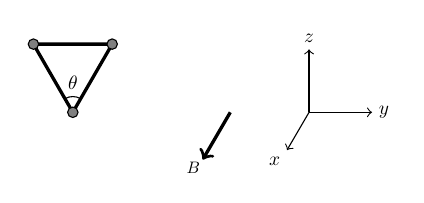
\begin{tikzpicture}
  \coordinate (H0) at (0, 0);
  \coordinate (H1) at ({sin(60/2)}, {cos(60/2)});
  \coordinate (H2) at ({-sin(60/2)}, {cos(60/2)});
  % =====================
  % Molecular arrangement
  % =====================
  \draw[very thick] (H1) -- (H0) -- (H2) -- cycle;
  \node[draw, shape=circle, fill=gray, scale=0.4] at (H0) {};
  \node[draw, shape=circle, fill=gray, scale=0.4] at (H1) {};
  \node[draw, shape=circle, fill=gray, scale=0.4] at (H2) {};
  \draw ({0.2*sin(60/2)}, {0.2*cos(60/2)}) arc [start angle=60, end angle=120, radius=0.2] node[anchor=south, midway, above, scale=.7] {$\theta$};
  % =====
  % Field
  % =====
  \draw[->, very thick] (2, 0) -- ++(-0.35, -0.6) node[scale=0.6, anchor=north east, inner sep=1pt] {$\symbfit{B}$};
  % =================
  % Coordinate system
  % =================
  \draw[->] (3, 0) -- ++(0.8, 0) node[anchor=west, scale=0.7] {$y$};
  \draw[->] (3, 0) -- ++(0, 0.8) node[anchor=south, scale=0.7] {$z$};
  \draw[->] (3, 0) -- ++(-0.28, -0.48) node[anchor=north east, scale=0.7] {$x$};
\end{tikzpicture}}
      \end{figure}

      \item<2-> Back-of-the-envelope properties for $\theta = 60\degree$:
      \begin{columns}[T]
        \begin{column}{.40\textwidth}
          \emphbf{red}{Zero field}
          \begin{itemize}
            \item<2-> Spatial sym. group: $\symcal{G} = \textcolor{red}{\symcal{D}_{3h}}$
          \end{itemize}
        \end{column}
        \begin{column}{.50\textwidth}
          \emphbf{blue}{Finite fields}
          \begin{itemize}
            \item<2-> Magnetic sym. group: $\symcal{M} = \textcolor{blue}{\symcal{D}_{3h}(\symcal{C}_{3h})}$
            \begin{itemize}
              \item Mag. unitary sym. subgroup: $\symcal{H} = \symcal{C}_{3h}$
              \item Spatial pseudo-sym. group: $\symcal{G} = \symcal{D}_{3h}$
            \end{itemize}
          \end{itemize}
        \end{column}
      \end{columns}

      \vspace{6	pt}

      \begin{columns}[T]
        \begin{column}{.40\textwidth}
          \begin{itemize}
            \item<3-> Ground term: \textcolor{red}{$E'(\symcal{D}_{3h})$}
          \end{itemize}
        \end{column}
        \begin{column}{.50\textwidth}
          \begin{itemize}
            \item<3-> Ground term: \textcolor{blue}{$\Gamma'(\symcal{C}_{3h})$} where
            \begin{equation*}
              \textcolor{red}{E'(\symcal{D}_{3h})} \to \textcolor{blue}{\Gamma'(\symcal{C}_{3h})} \oplus \bar{\Gamma}'(\symcal{C}_{3h})
            \end{equation*}
            \item<4-> Ground current: $\textcolor{blue}{A'(\symcal{C}_{3h})} \leftarrow \textcolor{red}{A_2'(\symcal{D}_{3h})}$
          \end{itemize}
        \end{column}
      \end{columns}
    \end{itemize}
    \footlessfullcite{article:Keith1993}
  \end{frame}


  %%%%%%%%%%%%%%%%%%%%%%%%%%
  %%%%%%%%%%%%%%%%%%%%%%%%%%
  \begin{frame}{Ground \glsfmtshort{acr:uhf} current density in \ce{H3} radical}
    \begin{itemize}
      \item<1-> \glsxtrshort*{acr:uhf}, 6-31G*, $M_S = -\nicefrac{1}{2}$
    \end{itemize}
    \only<1>{
      \begin{figure}
        \centering
        \animategraphics[controls, poster=first, scale=.7]{6}{./cursym/data/h3/h3.uhf.current.noint}{}{}
      \end{figure}
    }
    \only<2>{
      \begin{figure}
        \centering
        \animategraphics[controls, poster=first, scale=.7]{6}{./cursym/data/h3/h3.uhf.current.int}{}{}
      \end{figure}
    }
  \end{frame}

  %%%%%%%%%%%%%%%%%%%%%%%%%%
  %%%%%%%%%%%%%%%%%%%%%%%%%%
  \begin{frame}{Current density symmetry breaking}
    \begin{itemize}
      \only<1-2>{
        \item<1-> The ground \glsxtrshort*{acr:uhf} current density in equilateral \ce{H3} radical displays \emphit{Magenta}{symmetry breaking} at all $\lvert \gls*{mag:vec} \rvert/B_0 \in \interval[open left]{0}{1}$.\\[6pt]
        Current density symmetry analysis gives
        \begin{equation*}
          \textcolor{blue}{A' \oplus \Gamma' \oplus \bar{\Gamma}' (\symcal{C}_{3h})} \leftarrow \textcolor{red}{A_2' \oplus E' (\symcal{D}_{3h})}.
        \end{equation*}

        \item<2-> This suggests that the underlying \glsxtrshort*{acr:uhf} density and wavefunction are also symmetry-broken.
      }

      \only<3>{
        \item<3-> Consider the \glsxtrshort*{acr:uhf} wavefunction at $\lvert \gls*{mag:vec} \rvert = 0$:
        \begin{itemize}
          \item Overall symmetry: $A'_1 \oplus E' (\symcal{D}_{3h})$ $\Rightarrow$ \emphit{Magenta}{symmetry-broken}
          \item Occupied molecular-orbital isosurfaces at isovalues $\pm 0.1$:
          \begin{figure}
            \centering
            \captionsetup[subfigure]{labelformat=empty}
            \begin{subfigure}{.40\textwidth}
              \centering
              \phantom{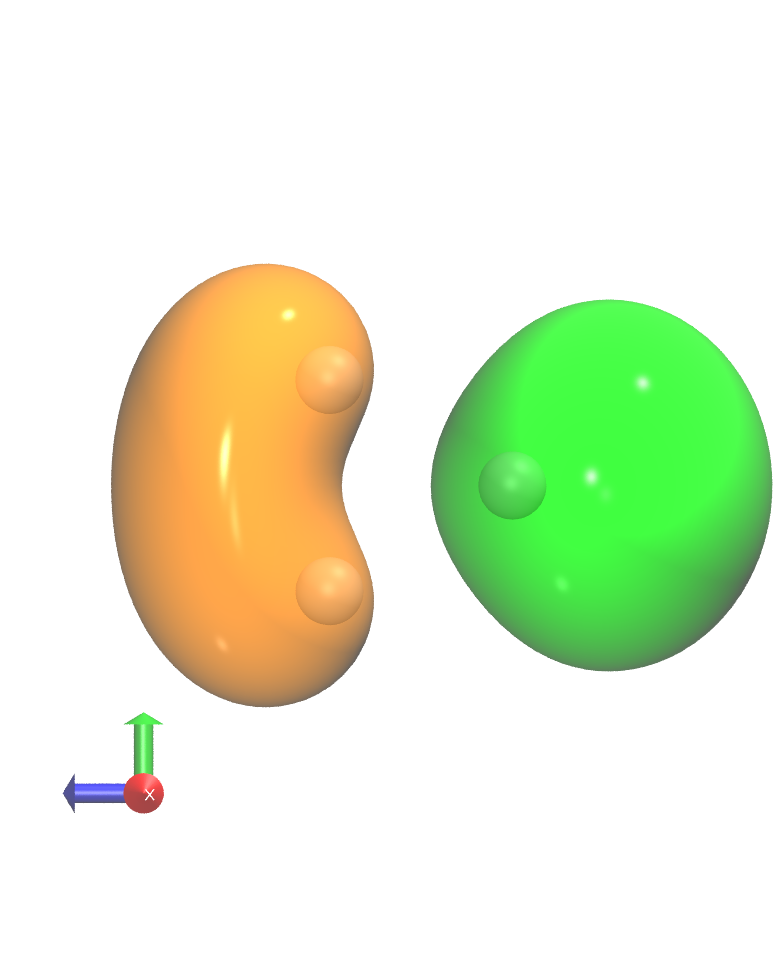
\includegraphics{./cursym/data/h3/b2_1200ppi.png}}
            \end{subfigure}
            \unskip\ \vrule\
            \begin{subfigure}{.40\textwidth}
              \centering
              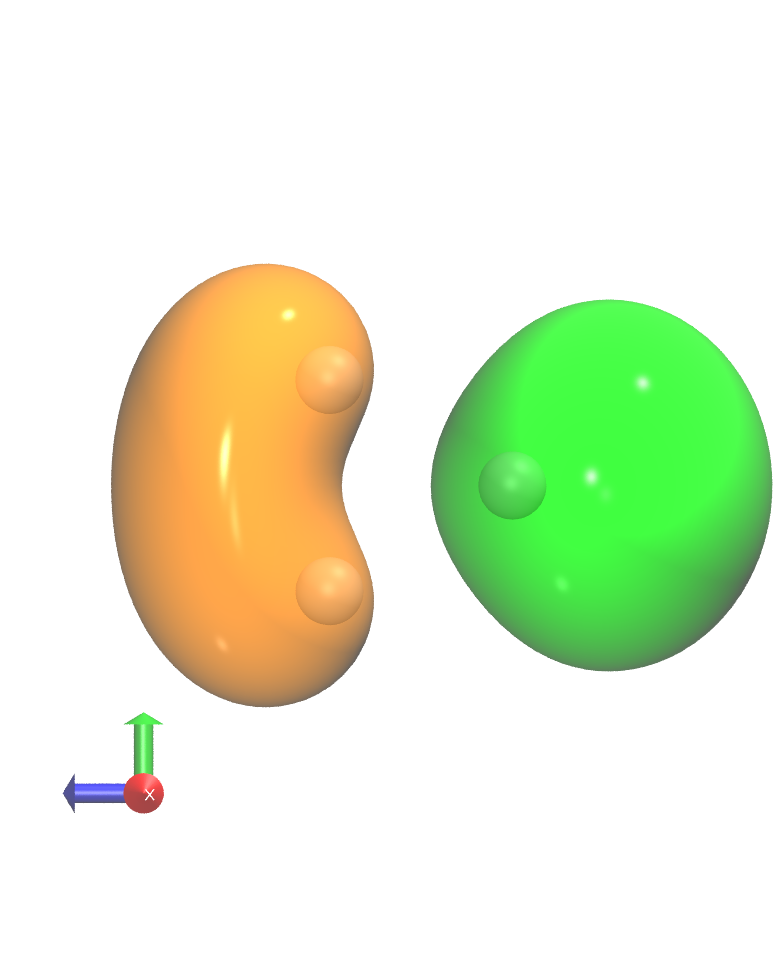
\includegraphics{./cursym/data/h3/b2_1200ppi.png}
              \subcaption{$\beta_2$, $A'_1 \oplus E' (\symcal{D}_{3h})$}
            \end{subfigure}

            \begin{subfigure}{.40\textwidth}
              \centering
              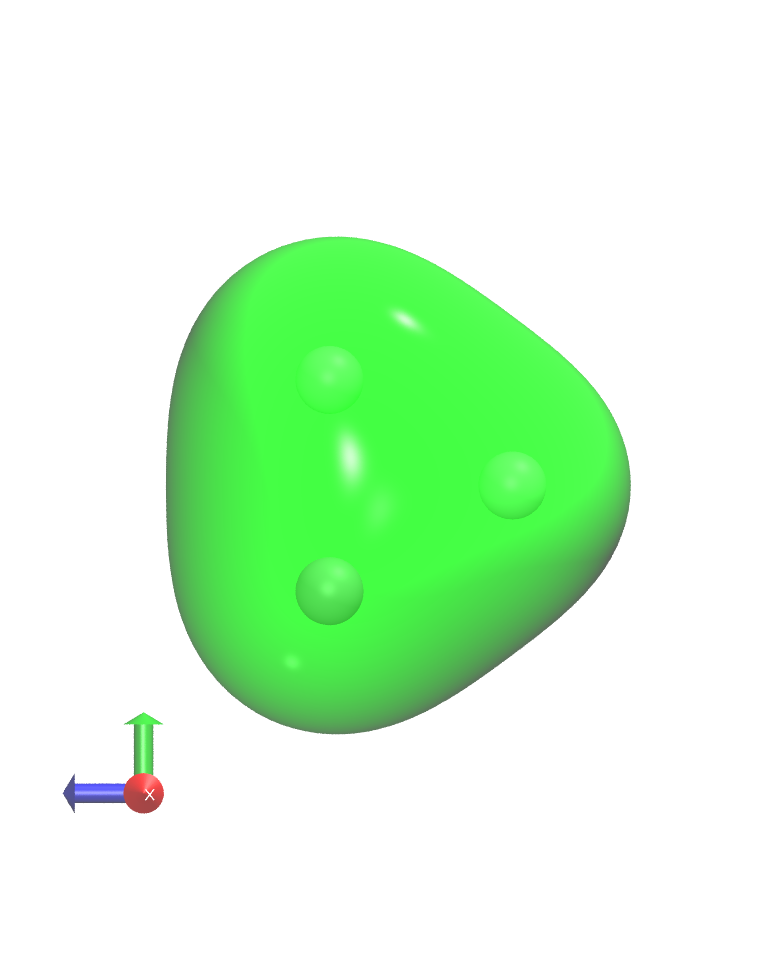
\includegraphics{./cursym/data/h3/a1_1200ppi.png}
              \subcaption{$\alpha_1$, $A'_1 \oplus E' (\symcal{D}_{3h})$}
            \end{subfigure}
            \unskip\ \vrule\
            \begin{subfigure}{.40\textwidth}
              \centering
              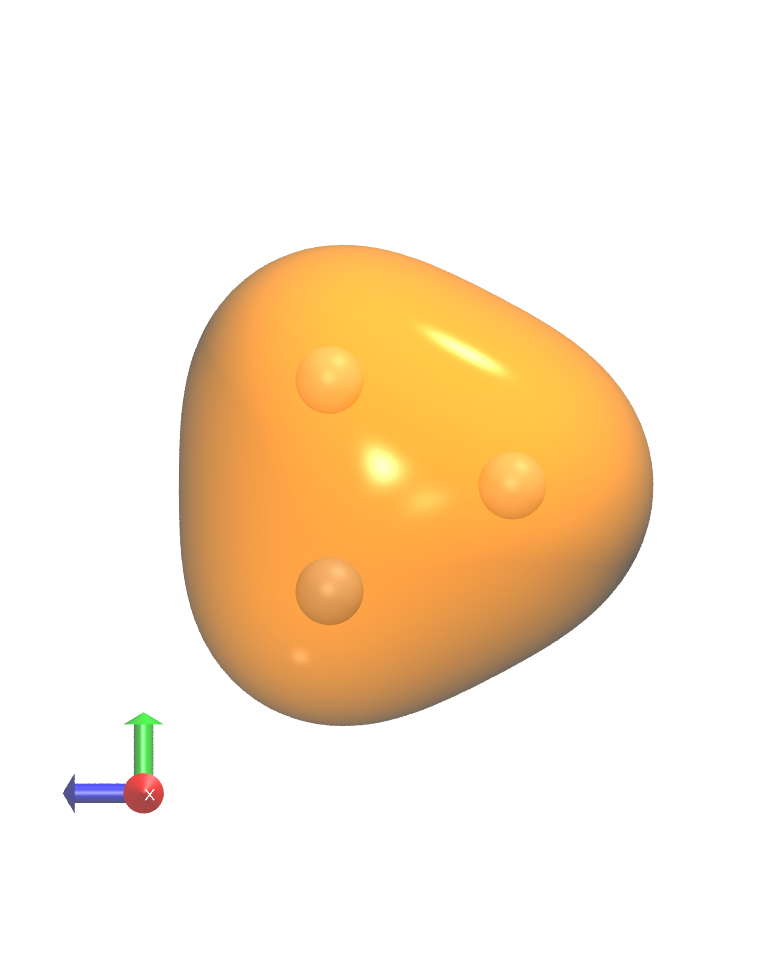
\includegraphics{./cursym/data/h3/b1_1200ppi.png}
              \subcaption{$\beta_1$, $A'_1 \oplus E' (\symcal{D}_{3h})$}
            \end{subfigure}
          \end{figure}
        \end{itemize}
      }

      \only<4->{
        \item<4-> This \glsxtrshort*{acr:uhf} symmetry breaking \emphit{Magenta}{persists} at finite field strengths:
        \begin{figure}
          \centering
          \pgfplotstableread[col sep=comma]{cursym/data/h3/h3.t60.000.csv}\data

\begin{tikzpicture}[%
]
  % Main plot
  \begin{groupplot}[
    % =============
    % Group configs
    % =============
    group style={
      group size=1 by 1,
      xlabels at=edge bottom,
      xticklabels at=edge bottom,
      ylabels at=edge left,
      yticklabels at=edge left,
      vertical sep=1.5cm,
      horizontal sep=1.8cm,
    },
    % =================
    % Groupplot general
    % =================
    width=.5\linewidth,
    scale only axis=true,
    cycle list name=coloronly,
    unbounded coords=jump,
    % ==================
    % Group title format
    % ==================
    title style={yshift=-1.5ex, font={\footnotesize}},
    % =================
    % Group axis format
    % =================
    % -----------------
    % Group axis scales
    % -----------------
    xmin=0, xmax=1,
    ymin=-1.725, ymax=-1.45,
    % -----------------
    % Group axis labels
    % -----------------
    xlabel={$\lvert \gls*{mag:vec} \rvert / B_0$},
    label style={font=\scriptsize},
    xlabel style={align=center},
    every axis y label/.append style={at={(0, 0.5)}, yshift=2.5em},
    % -----------------
    % Group tick labels
    % -----------------
    tick label style={font=\scriptsize},
    x tick label style=
    {
      /pgf/number format/.cd,
      fixed,
      fixed zerofill,
      precision=1,
      /tikz/.cd
    },
%    every y tick scale label/.style={%
%      at={(yticklabel cs:1)},%
%      anchor=east,%
%      inner sep=1pt%
%    },
    % ------------------
    % Group tick configs
    % ------------------
    xtick pos=left,
    xtick align=outside,
    minor x tick num=1,
    xtick distance=0.2,
    %%%%%%%%%%%%%%%%%%%%%%%%%%%%%
  ]
    % ==
    % ==
    % Wc
    % ==
    % ==
    % ------
    % Carbon
    % ------
    \nextgroupplot[
      % ===============
      % Subplot general
      % ===============
      align=center,
      ylabel={UHF energy / \si{\hartree}},
      height=.6\textheight,
      % ====================
      % Subplot title format
      % ====================
      % ===================
      % Subplot axis format
      % ===================
      % -------------------
      % Subplot axis scales
      % -------------------
      % -------------------
      % Subplot axis labels
      % -------------------
      y tick label style=
      {
        /pgf/number format/.cd,
        fixed,
        fixed zerofill,
        precision=2,
        /tikz/.cd
      },
      % -------------------
      % Subplot tick labels
      % -------------------
      % --------------------
      % Subplot tick configs
      % --------------------
      ytick align=outside,
      ytick pos=left,
      minor y tick num=1,
%      ytick distance=0.05,
      % ===============
      % Subplot legends
      % ===============
      legend pos=north east,
      legend style={
        legend cell align=right,
        legend style={font=\scriptsize},
      },
      % ===================
      % Subplot annotations
      % ===================
      after end axis/.code={%
        % ============
        % Point groups
        % ============
        \draw[<-, very thin] (rel axis cs:0, 1.015) -- ++(axis direction cs:0, 0.01) node[anchor=south, scale=0.5, inner sep=2pt] {$\symcal{D}_{3h}$};
        \node[anchor=south, scale=0.5, inner sep=2pt] at (rel axis cs:0.5, 1.020) {$\symcal{C}_{3h}$};
        % ===============
        % Symmetry labels
        % ===============
        \pgfplotstablegetelem{0}{s0_sym0_energy}\of{\data}
        \draw[very thin, ->] (axis cs:0, \pgfplotsretval) -- ++(axis direction cs:0.15, 0.01) node[anchor=west, scale=0.7, inner sep=2pt] {$A'_1 \oplus E' (\symcal{D}_{3h})$};
        \pgfplotstablegetelem{5}{s0_sym0_energy}\of{\data}
        \draw[very thin, ->] (axis cs:0.25, \pgfplotsretval) -- ++(axis direction cs:0.10, 0.025) node[anchor=south west, scale=0.7, inner sep=2pt] {$A' \oplus \Gamma' \oplus \bar{\Gamma}' (\symcal{C}_{3h})$};
      },
    ]
      \addplot[%
        DarkGreen,%
        smooth,
        very thick,%
        mark=none,%
      ] table[x={bx}, y={s0_sym0_energy}]{\data};
      \addlegendentry{$\gls*{wf:uhf}$}
      \addplot[%
        blue,%
        only marks,%
        mark=x,%
        mark size=2pt,%
      ] table[x={bx}, y={s0_sym1_energy}]{\data};
      \addlegendentry{$\hat{C}_3 \gls*{wf:uhf}$}
      \addplot[%
        red,%
        only marks,%
        mark=o,%
        mark size=1.5pt,%
      ] table[x={bx}, y={s0_sym2_energy}]{\data};
      \addlegendentry{$\hat{C}_3^{-1} \gls*{wf:uhf}$}
  \end{groupplot}
\end{tikzpicture}
        \end{figure}
      }
    \end{itemize}
  \end{frame}


  \subsection{\ce{H6} octahedron}
  %%%%%%%%%%%%%%%%%%%%%%%%%%
  %%%%%%%%%%%%%%%%%%%%%%%%%%
  \begin{frame}{Degenerate current density symmetry}
    \begin{itemize}
      \item<1-> Consider an octahedral \ce{H6} cluster.
      \begin{figure}
        \centering
        \scalebox{.8}{\ifdefined\molsize
  \setlength{\molsize}{1.2cm}
\else
  \newlength{\molsize}
  \setlength{\molsize}{1.2cm}
\fi
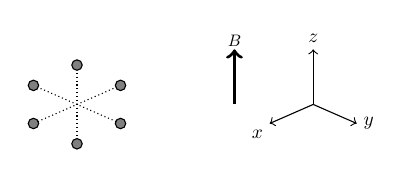
\begin{tikzpicture}
  \coordinate (top) at (0, 0.50\molsize);
  \coordinate (bottom) at (0, -0.50\molsize);
  \coordinate (topleft) at (-0.553\molsize, 0.242\molsize);
  \coordinate (bottomleft) at (-0.553\molsize, -0.242\molsize);
  \coordinate (topright) at (0.553\molsize, 0.242\molsize);
  \coordinate (bottomright) at (0.553\molsize, -0.242\molsize);
  % =====================
  % Molecular arrangement
  % =====================
  \draw[densely dotted] (top) -- (bottom);
  \draw[densely dotted] (topleft) -- (bottomright);
  \draw[densely dotted] (topright) -- (bottomleft);
  \node[draw, shape=circle, fill=gray, scale=0.4] at (top) {};
  \node[draw, shape=circle, fill=gray, scale=0.4] at (bottom) {};
  \node[draw, shape=circle, fill=gray, scale=0.4] at (topleft) {};
  \node[draw, shape=circle, fill=gray, scale=0.4] at (bottomleft) {};
  \node[draw, shape=circle, fill=gray, scale=0.4] at (topright) {};
  \node[draw, shape=circle, fill=gray, scale=0.4] at (bottomright) {};
  % =====
  % Field
  % =====
  \draw[->, very thick] (2, 0) -- ++(0, 0.7) node[scale=0.6, anchor=south, inner sep=1pt] {$\symbfit{B}$};
  % =================
  % Coordinate system
  % =================
  \draw[->] (3, 0) -- ++(0.553, -0.242) node[anchor=west, scale=0.7] {$y$};
  \draw[->] (3, 0) -- ++(0, 0.7) node[anchor=south, scale=0.7] {$z$};
  \draw[->] (3, 0) -- ++(-0.553, -0.242) node[anchor=north east, scale=0.7] {$x$};
\end{tikzpicture}}
      \end{figure}

      \item<1-> Back-of-the-envelope properties for $\gls*{mag:vec}$ along $z$:
      \begin{columns}[T]
        \begin{column}{.40\textwidth}
          \emphbf{red}{Zero field}
          \begin{itemize}
            \item<1-> Spatial sym. group: $\symcal{G} = \textcolor{red}{\symcal{O}_{h}}$
          \end{itemize}
        \end{column}
        \begin{column}{.50\textwidth}
          \emphbf{blue}{Finite fields}
          \begin{itemize}
            \item<1-> Magnetic sym. group: $\symcal{M} = \textcolor{blue}{\symcal{D}_{4h}(\symcal{C}_{4h})}$
            \begin{itemize}
              \item Mag. unitary sym. subgroup: $\symcal{H} = \symcal{C}_{4h}$
              \item Spatial pseudo-sym. group: $\symcal{G} = \symcal{O}_{h}$
            \end{itemize}
          \end{itemize}
        \end{column}
      \end{columns}

      \vspace{6pt}

      \begin{columns}[T]
        \begin{column}{.40\textwidth}
        \end{column}
        \begin{column}{.50\textwidth}
          \begin{itemize}
            \item<1-> Ground current: $\textcolor{blue}{A_g(\symcal{C}_{4h})} \leftarrow \textcolor{red}{T_{1g}(\symcal{O}_{h})}$
          \end{itemize}
        \end{column}
      \end{columns}
    \end{itemize}
  \end{frame}


  %%%%%%%%%%%%%%%%%%%%%%%%%%
  %%%%%%%%%%%%%%%%%%%%%%%%%%
  \begin{frame}{Principal-field current density in \ce{H6} cluster}
    \begin{columns}
      \begin{column}{.40\textwidth}
        \begin{itemize}
          \setlength\itemsep{1.2em}
          \item<1-> \glsxtrshort*{acr:uhf}, 6-31G*, $M_S = 0$
          \item<1-> $\gls*{mag:vec}$ along $z$-direction
          \item<1-> $\gls*{mag:jphys}(\gls*{bas:spatialcoord})$ symmetry: $\textcolor{blue}{A_g(\symcal{C}_{4h})} \leftarrow \textcolor{red}{T_{1g}(\symcal{O}_{h})}$
          \item<1-> \glsxtrshort*{acr:uhf} symmetry: $B_g(\symcal{C}_{4h})$
        \end{itemize}
      \end{column}

      \begin{column}{.55\textwidth}
        \begin{figure}
          \centering
          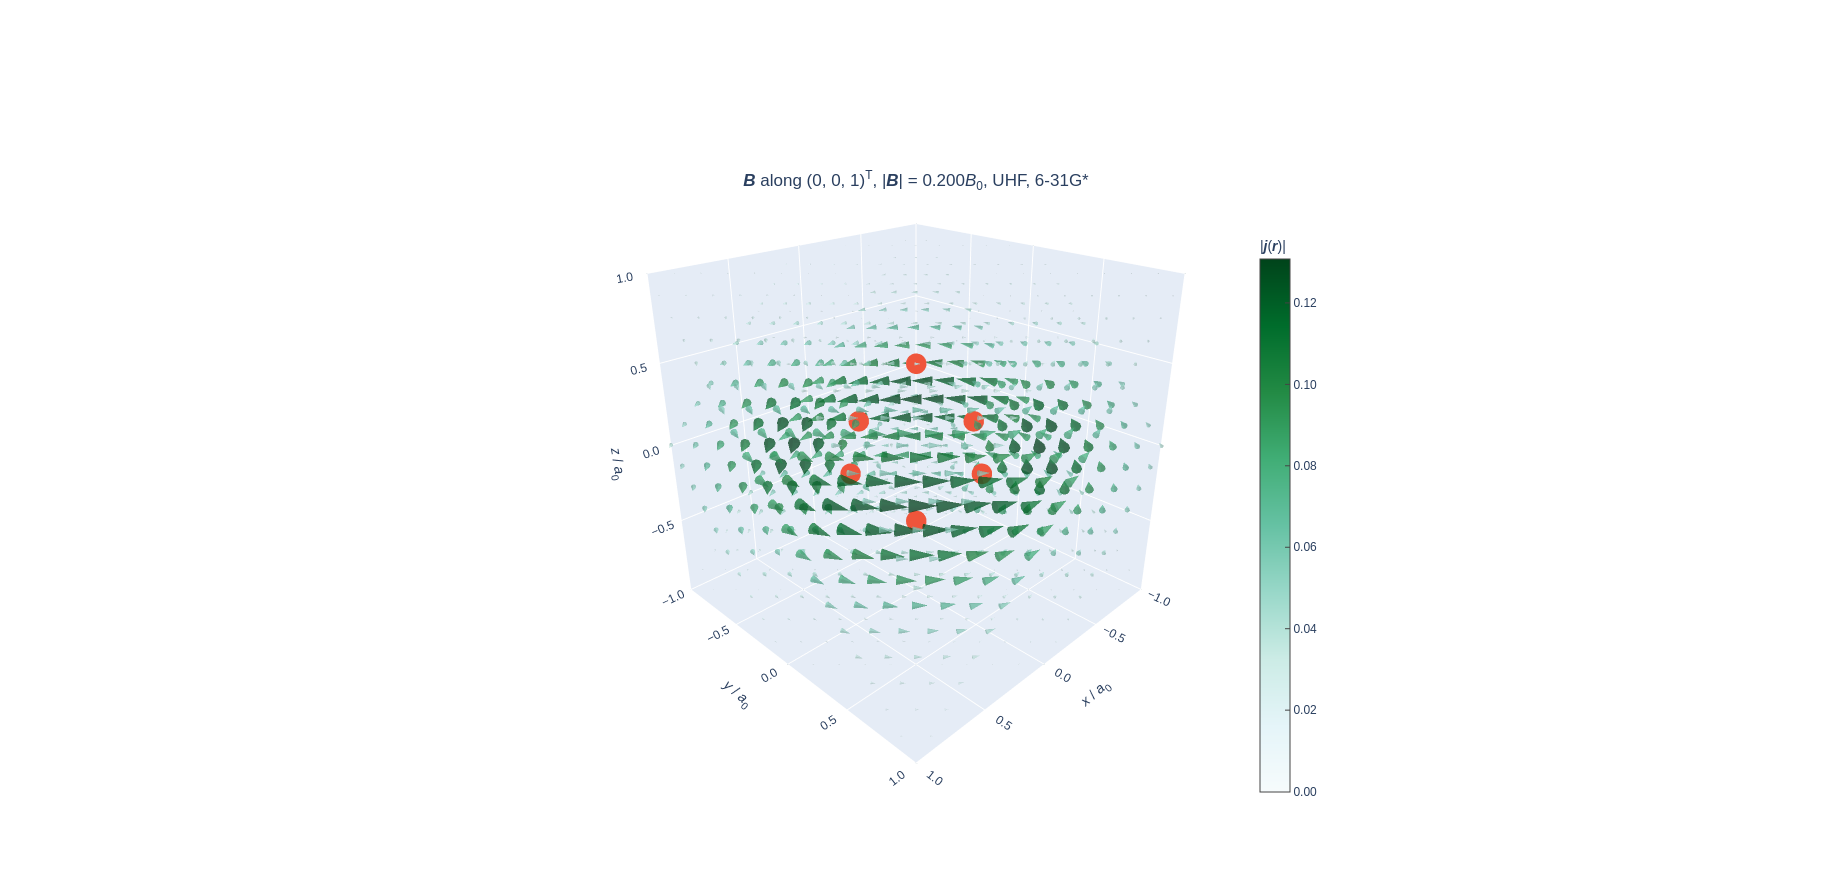
\includegraphics[trim=600 50 500 150, clip, width=\textwidth]{./cursym/data/h6/bz.png}
        \end{figure}
      \end{column}
    \end{columns}
  \end{frame}


  %%%%%%%%%%%%%%%%%%%%%%%%%%
  %%%%%%%%%%%%%%%%%%%%%%%%%%
  \begin{frame}{Non-principal-field current density in \ce{H6} cluster}
    \begin{columns}
      \begin{column}{.40\textwidth}
        \begin{itemize}
          \setlength\itemsep{1.2em}
          \item<1-> \glsxtrshort*{acr:uhf}, 6-31G*, $M_S = 0$
          \item<1-> $\gls*{mag:vec}$ along $(1, 1, 1)^{\T}$ direction
          \item<1-> $\gls*{mag:jphys}(\gls*{bas:spatialcoord})$ symmetry: $\textcolor{blue}{A_g(\symcal{S}_{6})} \leftarrow \textcolor{red}{\underline{T_{1g}} \oplus A_{2g}(\symcal{O}_{h})}$
          \item<1-> \glsxtrshort*{acr:uhf} symmetry: $\bar{\Gamma}_g(\symcal{S}_{6})$
        \end{itemize}
      \end{column}

      \begin{column}{.55\textwidth}
        \begin{figure}
          \centering
          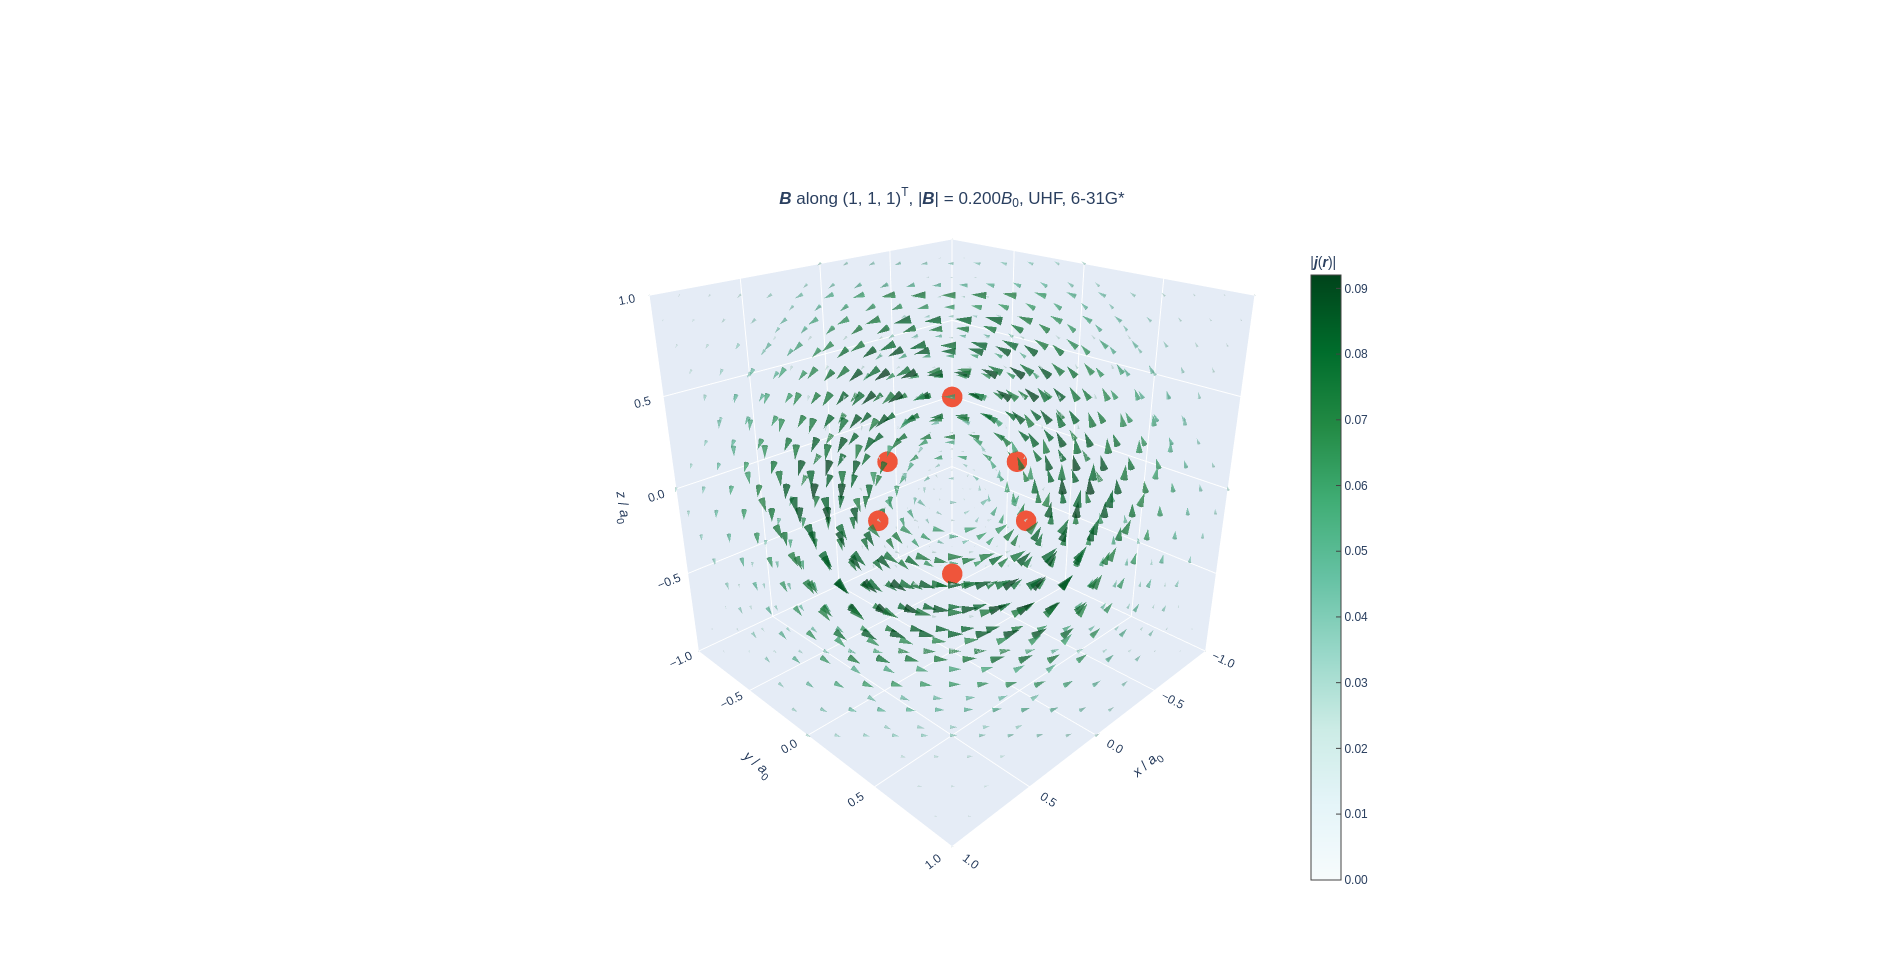
\includegraphics[trim=600 50 500 150, clip, width=\textwidth]{./cursym/data/h6/bxyz.png}
        \end{figure}
      \end{column}
    \end{columns}
  \end{frame}